\documentclass[11pt]{article}
\usepackage[margin=2.2cm]{geometry}
\usepackage{graphicx}
\usepackage{amsmath}
\usepackage{booktabs}
\usepackage{caption}
\usepackage{xcolor}
\usepackage[authoryear,round]{natbib}
\usepackage[hidelinks]{hyperref}

% Figure paths are relative to this directory (paper/jomission_lansa); result files live at ../../results/.
% A missing file renders a boxed "pending" stub instead of failing the build.
\newcommand{\todo}[1]{\textcolor{red}{\textbf{[TODO: #1]}}}
\newcommand{\pendingbox}[1]{\fbox{\begin{minipage}[c][3.2cm][c]{0.92\linewidth}\centering\small\textbf{pending:} #1\end{minipage}}}
% #1 panel letter, #2 file (relative path), #3 width, #4 text of the pending stub
\newcommand{\panel}[4]{%
  \begin{minipage}[t]{#3}\centering
  \IfFileExists{#2}{\includegraphics[width=\linewidth]{#2}}{\pendingbox{#4}}\\[0.3em]
  \textbf{#1}
  \end{minipage}}

\title{Laminar-cellular architecture sets the spectrolaminar motif in a primate model of the cortical hierarchy}
\author{\todo{author list}}
\date{Skeleton draft, 2026-11-10}

\begin{document}
\maketitle

\begin{abstract}
\todo{abstract: question, model, readouts and result, written only after the results it summarizes exist}
\end{abstract}

\section{Introduction}

The spectrolaminar motif is depth-resolved power: alpha-beta peaks in deep layers and gamma in superficial
layers, with a crossing between them \citep{MendozaHalliday2024}.
\todo{state the motif definition and the observed finding exactly as MendozaHalliday2024 gives them; check against the source}

\todo{the cortical hierarchy and the laminar question; what prior modelling of laminar spectra showed, including the
SLM model paper \citep{Herrera2026}, whose gamma-source view differs from this project's (docs/laminar\_motif/PLAN\_LANSA\_E2.md)}

We ask which laminar-cellular features of a three-unit JaxFNE stack set the motif. The estimand, the
readouts and the test designs are in Methods. \todo{one-paragraph claim, stated after the seals are frozen}

\section{Results}

% Result text is placeholder until its seal's run completes. No result number appears here unless it is copied
% from a named file, and that file is cited in a comment beside it.
% Figure files are referenced by relative path (../../results/...). A missing file renders a pending stub.
\newcommand{\stub}[2]{\begin{minipage}[t]{0.48\linewidth}\centering\pendingbox{#2}\\[0.3em]\textbf{#1}\end{minipage}}

\subsection{Fig 1: reference model}

\begin{figure}[tbp]
\centering
\IfFileExists{../../results/viz/schema/t1_kd1p41_n4000_s1_T8_schema.png}{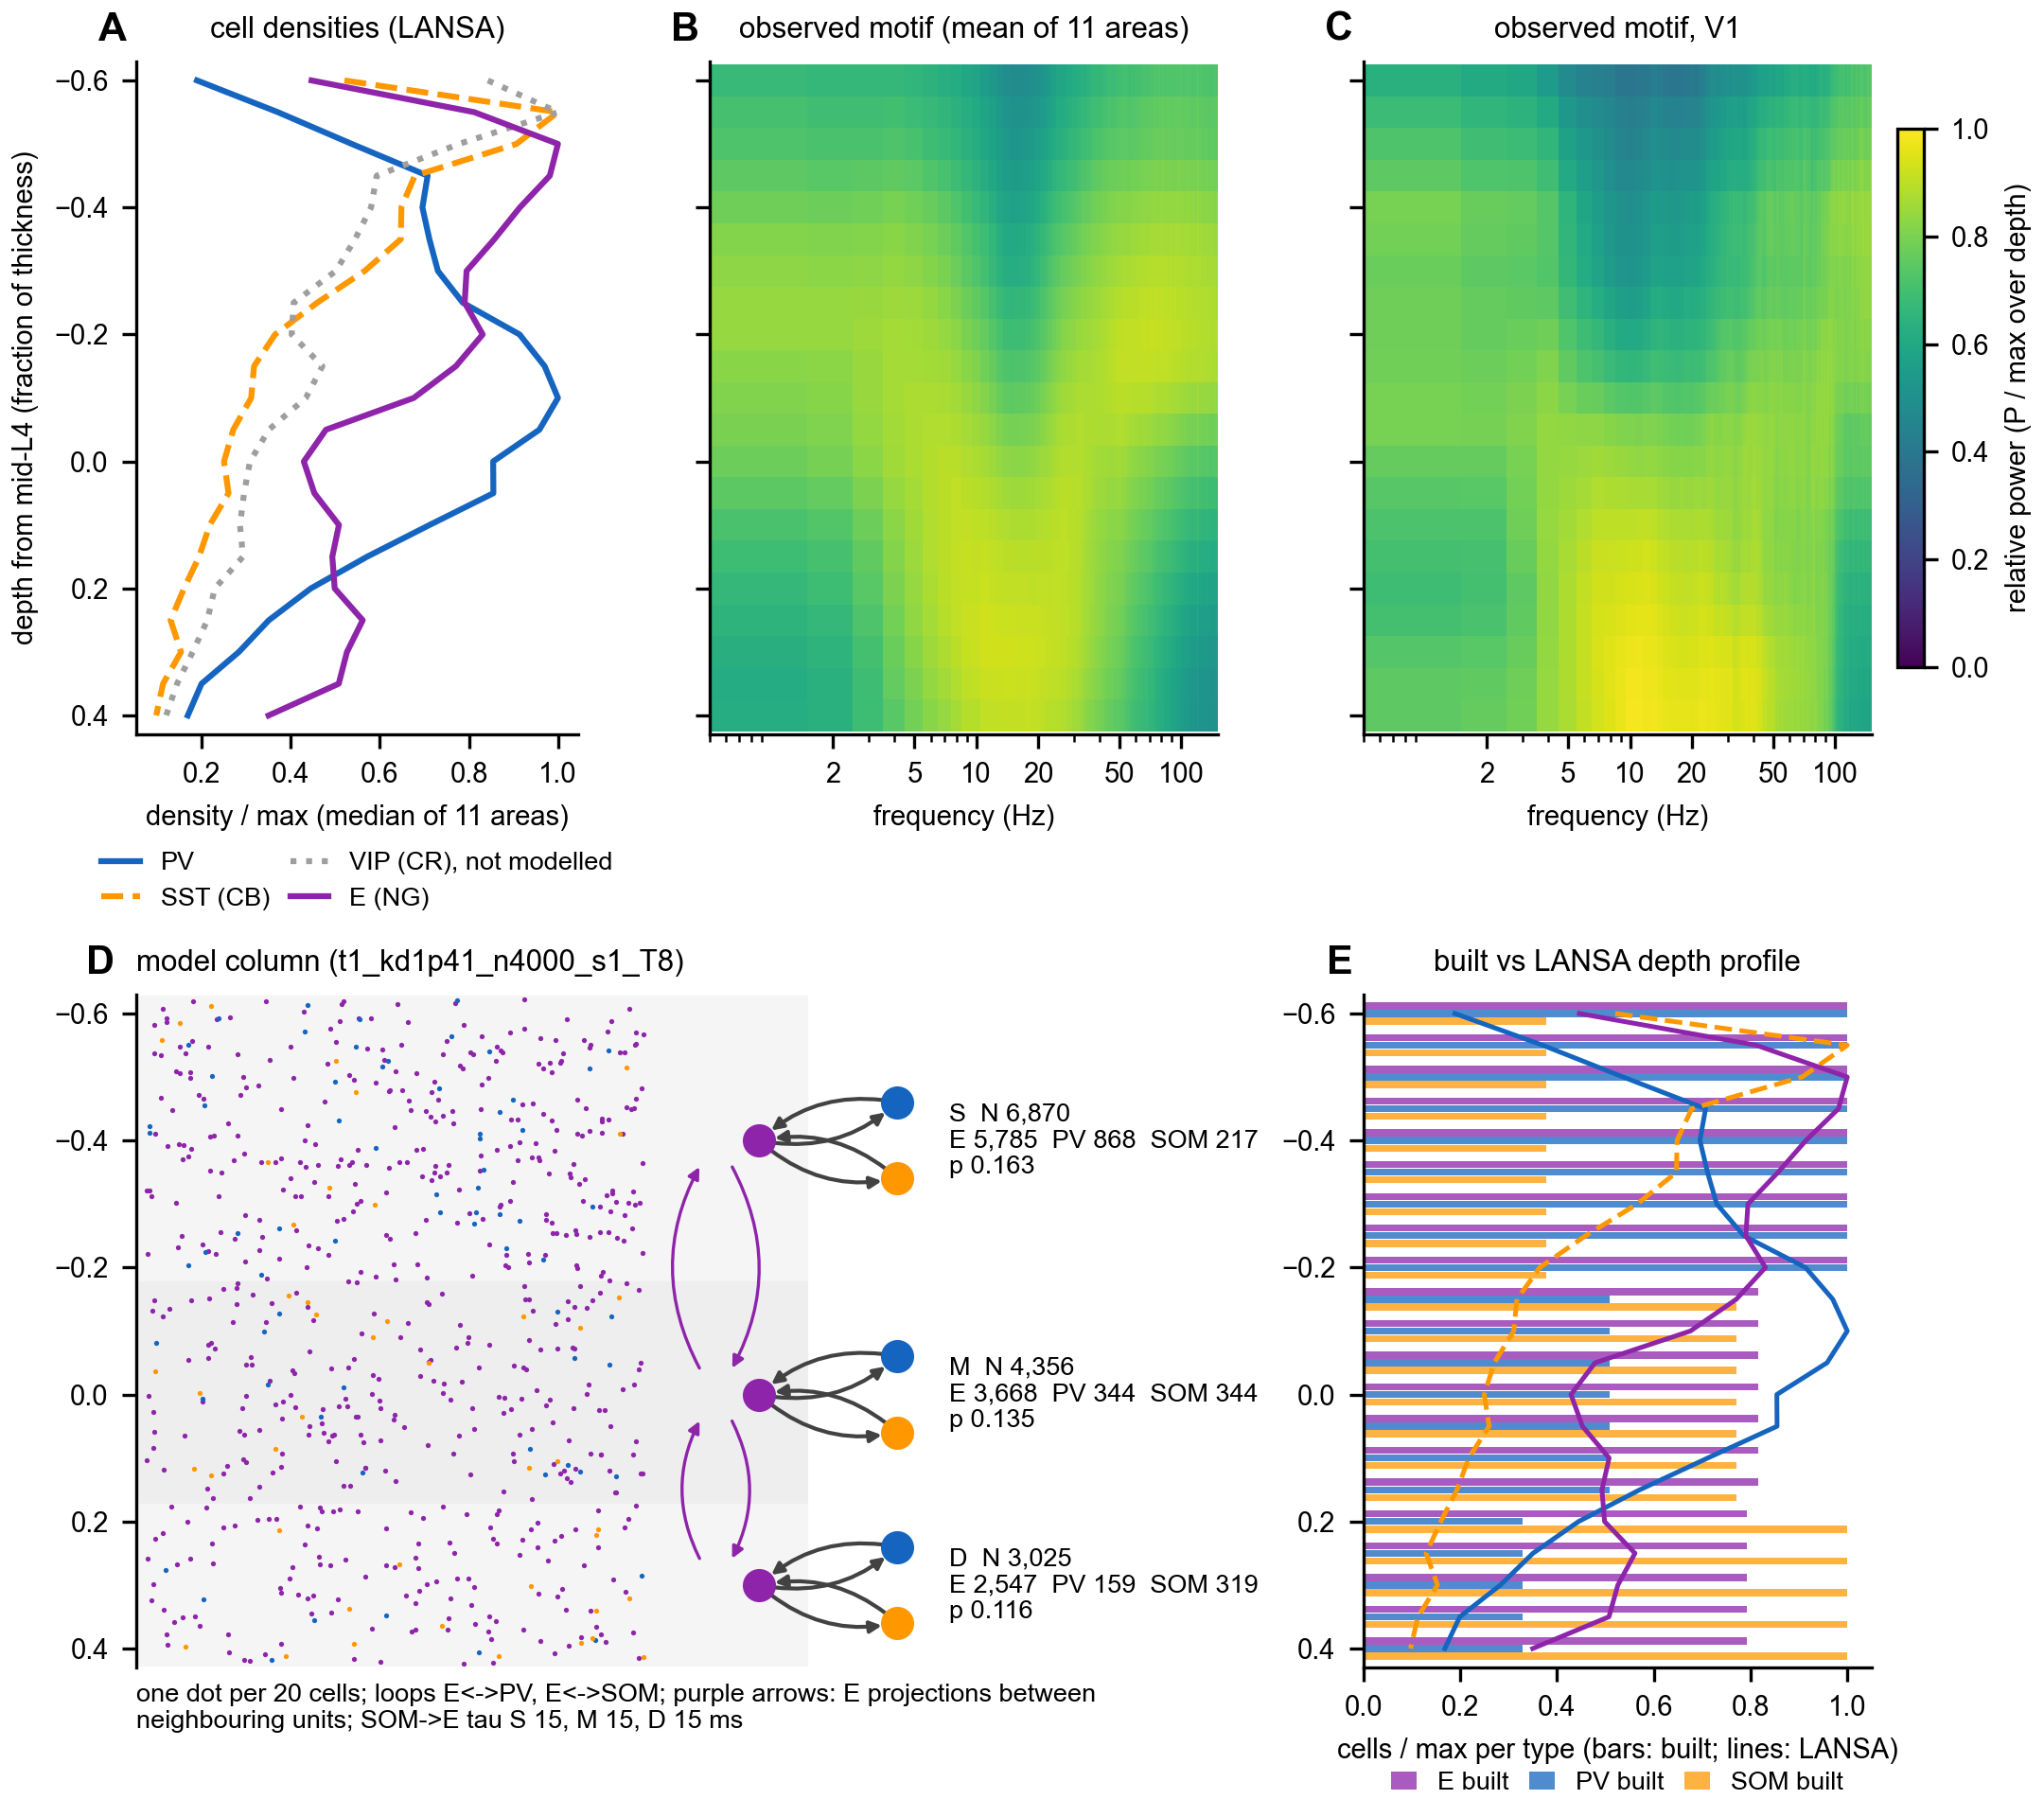
\includegraphics[width=\linewidth]{../../results/viz/schema/t1_kd1p41_n4000_s1_T8_schema.png}}{\pendingbox{data and circuit schema}}
\caption{Data and circuit (layout after Herrera 2026; \texttt{scripts/e2\_circuit\_schema.py}). A: LANSA cell densities
per type against depth from mid-L4, median of 11 areas, each type divided by its maximum (CB taken as SST, CR as VIP,
NG as the pyramidal proxy). B, C: observed relative power, mean of the 11 areas and V1. D: the T1 model
(\texttt{e2\_3unit\_n4000\_dens\_k1\_kd1p41\_sst15}) as built, one dot per 20 cells in each unit's depth bins, with its
within-unit loops and inter-unit E projections. E: built cells per type and depth bin against the LANSA profiles. LANSA
densities are relative per type, so E compares depth profiles only. No panel is simulated.}
\end{figure}

\todo{Fig 1 text: the reference model kd1\_sst15 at n4000, seed 1; its architecture, raster, spectra, SL maps, LFP and CSD; the observed LANSA map.}

\begin{figure}[tbp]
\centering
\panel{A}{../../results/viz/paper_w3/sw_n4000_dens_k1_kd1_sst15_s1_T8_V0_architecture.png}{0.85\linewidth}{V0 architecture}
\caption{Reference model \texttt{e2\_3unit\_n4000\_dens\_k1\_kd1\_sst15}, seed 1, 8 s run, 2 s discarded; an exploratory
E2 run (see the software status in Methods). A: architecture from the V0 file (paper\_w3). The details table (cell
numbers and types per unit, edges per rule, parameters with their sources) is Tables~S1--S4.}
\end{figure}

\begin{figure}[tbp]
\centering
\IfFileExists{../../results/viz/paper_w3/sw_n4000_dens_k1_kd1_sst15_s1_T8_block.png}{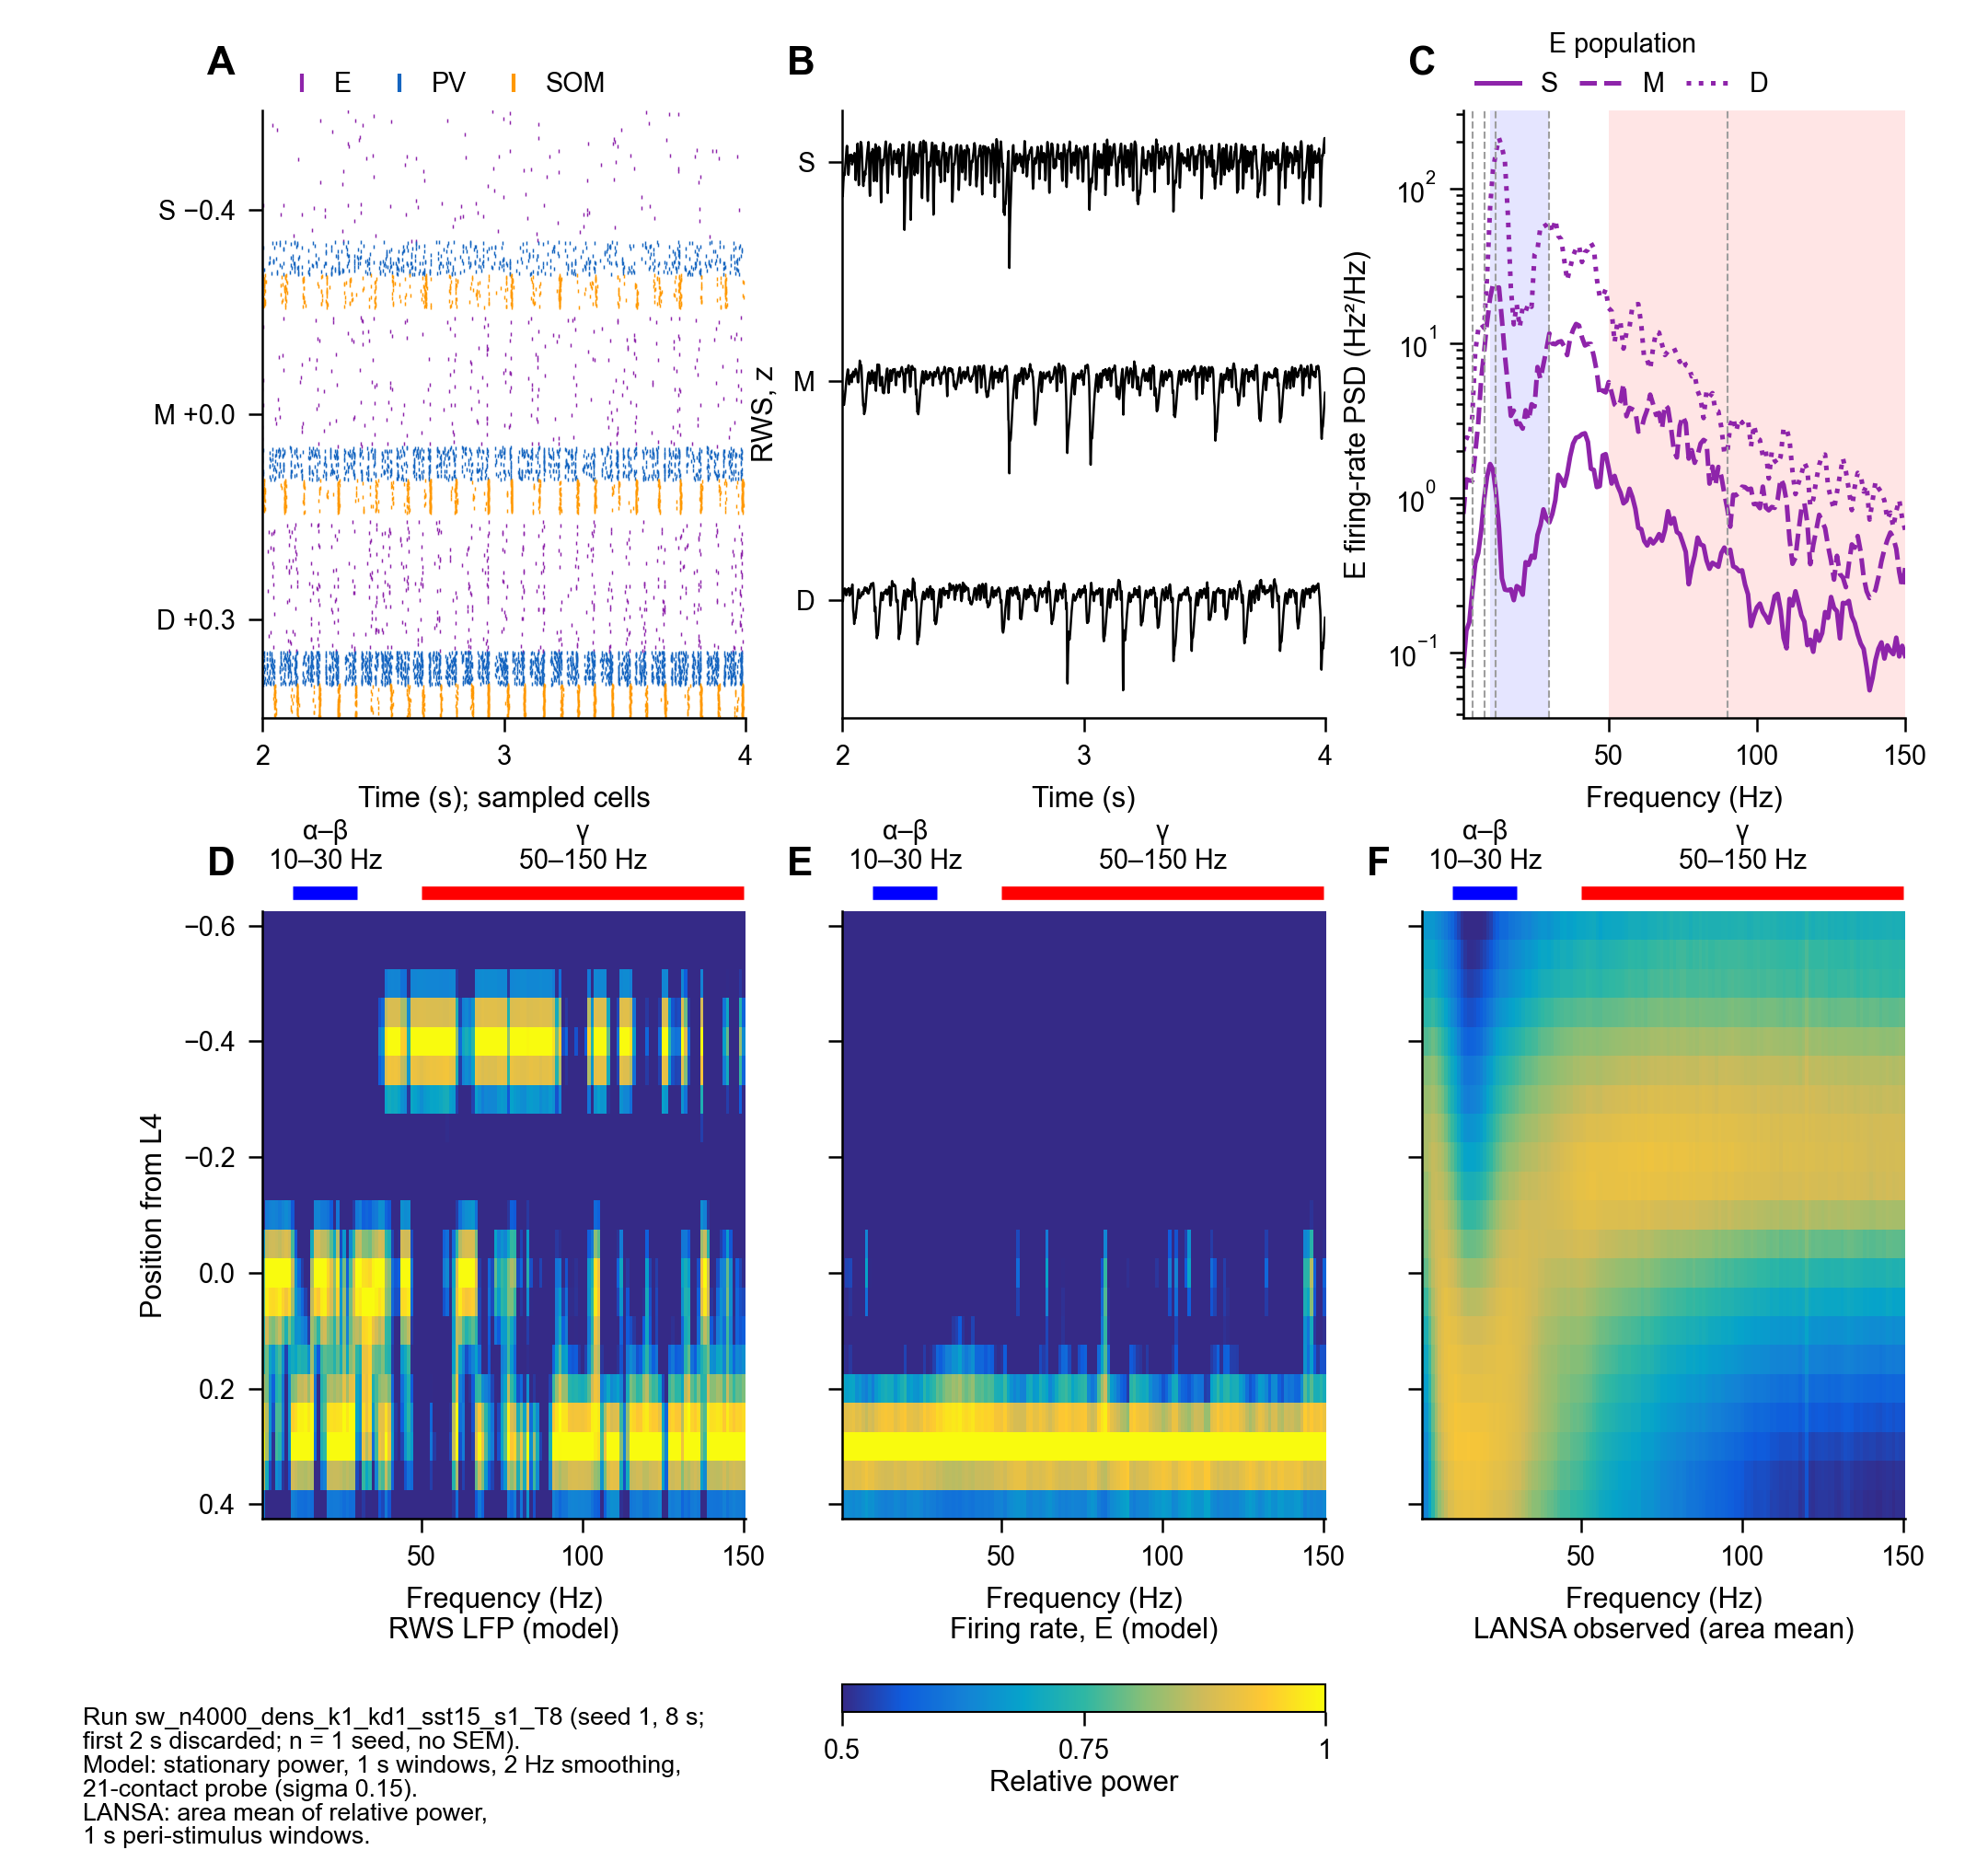
\includegraphics[width=\linewidth]{../../results/viz/paper_w3/sw_n4000_dens_k1_kd1_sst15_s1_T8_block.png}}{\pendingbox{block figure}}
\caption{Reference model, seed 1 (block file, paper\_w3). Its panels are mapped to the plan: file A (raster) = Fig 1B;
file C (per-type spectra) = Fig 1C; files D (RWS SL map) and E (firing-rate SL map) = Fig 1D; file F (observed LANSA
area map) = Fig 1E. File B (RWS traces) is not a plan panel. The letters in the image are the file's own.}
\end{figure}

\begin{figure}[tbp]
\centering
\panel{F}{../../results/laminar_e2/sw_n4000_dens_k1_kd1_sst15_s1_T8_motif.png}{0.48\linewidth}{LFP proxy and band-depth profiles}
\hfill
\panel{F (CSD)}{../../results/viz/paper_w4/sw_n4000_dens_k1_kd1_sst15_s1_T8_csd.png}{0.48\linewidth}{current-based CSD}
\caption{Reference model, seed 1. F: LFP proxy traces and band-depth profiles from the motif file (its panels d--i).
Current-based CSD from paper\_w4; CSD placements are ASSUMED (Methods). Panel letters in the image files are their own.}
\end{figure}

\subsection{Fig 2: robustness}

\todo{Fig 2 text: drive-rate sweep and seed robustness as difference maps with SSIM and Pearson r; the hierarchy panel is deferred (T7, plan section 5).}

\begin{figure}[tbp]
\centering
\stub{A: drive-rate sweep difference maps (SSIM, r)}{drive-rate sweep difference maps (SSIM, Pearson r); no difference maps written yet}
\hfill
\panel{B}{../../results/viz/paper_w6/seed_diff.png}{0.48\linewidth}{seed difference maps}\\[0.8em]
\stub{C: LANSA hierarchy (T7)}{T7 LANSA hierarchy, deferred (plan section 5, OPEN-38)}
\caption{Robustness. A: drive-rate sweep, not written. B: seed difference maps $R_a - R_b$ of the relative-power map
for each pair of seeds 1--3 at $N$ = 1000, 2000, 4000 (ladder runs), with SSIM and Pearson $r$ over all pixels
(\texttt{paper\_w6/seed\_diff.png}). Seed pairs agree (SSIM 0.62--0.71, $r$ 0.87--0.93); each seed against the
observed map gives SSIM 0.04--0.12 and $r$ 0.20--0.43. Panel C is deferred.}
\end{figure}

\subsection{Fig 3: interneuron manipulations}

\todo{Fig 3 text: PV and SST silencing, whole population and per unit; PV/SST ratio scale; VIP is stage 2.}

\begin{figure}[tbp]
\centering
\stub{A: PV silencing, whole population}{T4 PV silencing, whole population (not run)}
\hfill
\stub{B: SST silencing, whole population}{T4 SST silencing, whole population (not run)}\\[0.8em]
\stub{C: silencing per unit}{T4 per-unit silencing (not run)}
\hfill
\stub{D: PV/SST ratio scale}{T3 PV/SST ratio scale (not run)}\\[0.8em]
\stub{E: VIP}{T5 VIP, stage 2 (deferred, OPEN-36)}
\caption{Interneuron manipulations. All panels are pending; the T4 and T3 seals are in \texttt{docs/laminar\_motif/}.}
\end{figure}

\subsection{Fig 4: laminar source}

\todo{Fig 4 text: unit silencing, isolated units, graded PV silencing inside the isolated gamma unit.}

\begin{figure}[tbp]
\centering
\stub{A: unit silencing}{T4 unit silencing (not run)}
\hfill
\stub{B: isolated units}{isolated-unit runs (not run)}\\[0.8em]
\stub{C: graded PV silencing, isolated gamma unit}{graded fractions 10/25/50/75/100\% (deferred; sub-population label not built)}
\caption{Laminar source. All panels are pending.}
\end{figure}

\subsection{Fig 5: determinants}

\todo{Fig 5 text: S$\leftrightarrow$D swaps of $\rho$, in-degree, N and SST$\to$E $\tau$ on isolated units; E/I $g$ in $\{0.5, 2\}$.}

\begin{figure}[tbp]
\centering
\stub{A: S$\leftrightarrow$D swap, $\rho$}{swap of rho on isolated units (not run)}
\hfill
\stub{B: S$\leftrightarrow$D swap, in-degree}{swap of in-degree (not run)}\\[0.8em]
\stub{C: S$\leftrightarrow$D swap, N}{swap of N (not run)}
\hfill
\stub{D: SST$\to$E $\tau$}{swap of SST$\to$E $\tau$ (not run)}\\[0.8em]
\stub{E: E/I $g$}{T2 E/I, $g$ in $\{0.5, 2\}$ (not run)}
\caption{Determinants. All panels are pending.}
\end{figure}

\subsection{Fig 6: probe geometry}

\todo{Fig 6 text: tilted and offset probe readouts, scored by contrast M and by $r_\text{proto}$ minus the identical-unit control (T6; readout only, no simulation).}

\begin{figure}[tbp]
\centering
\panel{A}{../../results/viz/paper_w5/sw_n4000_dens_k1_kd1_sst15_s1_T8_probe_geometry.png}{0.48\linewidth}{probe geometry}
\hfill
\panel{B}{../../results/viz/paper_w5/lfs_n1000_s1_T8_probe_geometry.png}{0.48\linewidth}{probe geometry, n1000}\\[0.8em]
\panel{C}{../../results/viz/paper_w5/probe_summary.png}{0.96\linewidth}{T6 score summary by $\theta$ and offset}
\caption{Probe geometry, post hoc readout on saved runs. A: reference model; B: n1000 seed 1 (W5 readout outputs).
C: contrast $M_\text{arc}$ and $r_\text{proto} - r_\text{ctrl}$ by tilt and lateral offset, seed mean $\pm$ SD over
seeds 1--3 at each $N$ (\texttt{probe\_summary.png}). At offsets 0 and 0.25 the rise of $r_\text{proto} - r_\text{ctrl}$
with tilt comes from the identical-unit control falling, not from $r_\text{proto}$, which falls at $\theta = 30^\circ$.}
\end{figure}

\section{Discussion}

A column sized from LANSA cell densities, with an imposed SOM/PV ramp, and a CAMINOS module that reproduces its reference placed alpha-beta in
its deep half on its selection seeds, with the band profiles crossing on 2 of 3, but left relative gamma between $-0.2$ and 0
of cortical thickness at a quarter to a third of the observed level, where the observed gamma is broadest. No run passed the shared scorer: not the nine ladder runs, not the
63 level-seed scores of the sealed search, and not the frozen winner on three fresh seeds. Every ladder and T1 run
failed the gamma depth criterion; only exploratory weight runs reached it, each losing the alpha-beta criterion or
the crossing. The alpha-beta criterion held for the reference column at $N = 4000$ on its three selection seeds
(in-sample; the reference was not rerun on fresh seeds), but not for the T1 winner, on its own selection seeds
(0.32--0.47) or on fresh seeds (0.35--0.47), so deep alpha-beta is reproduced only in part. At the declared unit depths the readout
kernel is not the limit (ceilings 0.854 and 0.693), but moving the depths changes the scores substantially
(Results), so readout depth remains a confound rather than a ruled-out cause. The drop in $r_{ab}$ from the reference
(0.83--0.86) to the T1 winner (0.32--0.47) is itself a primary result: the alpha-beta placement of the reference
does not survive the sealed tuning, which selected on $r_\text{proto}$.

The negative result is specific. It holds for this three-unit E/PV/SOM column with density-scaled sizes and
in-degrees, the declared SOM/PV ramp, the tested SOM$\to$E kinetics and network sizes, and stationary drive. It does
not show that density-based or CAMINOS-based models in general cannot produce the motif, and it does not test, so
cannot contradict, the PV$\to$E kinetics that \citet{Herrera2026} found to control layer-4 gamma. What it shows is
that densities and SOM kinetics alone were not sufficient here. The sealed controls separate the two construction
inputs. The deep alpha-beta follows the imposed SOM/PV ramp: flattening or reversing it moved alpha-beta
superficial on every seed, while flattening the density profile left it in place. The density profile shapes the
gamma profile and the whole map: flattening or permuting it turned $r_{gm}$ and $r_\text{proto}$ negative. The
model's best feature, deep alpha-beta, therefore rests on the declared ratio ramp, which runs against the measured
CB/PV profile, rather than on the measured densities. The controls do not identify a band-specific mechanism:
each arm let one unit dominate the map at every frequency, and they change sizes, in-degrees and rates along with
the named quantity.

\textbf{What is missing.} The first explanation is a band mismatch, and it may be the central one. The isolated
CAMINOS module oscillates at 27--46 Hz depending on $\rho$, below the scored 50--150 Hz band, and in the stack the
M and D units peak at 11--12 Hz. The model may therefore lack a strong oscillatory mode in the scored band at
any depth, not merely place one at the wrong depth: its relative 50--150 Hz power comes from the tails of these
rhythms and from S, not from a dedicated fast generator, and because power is normalized per frequency across depth, weak mid-depth values can
also reflect excess S or D power rather than missing M power. A model built from this module may need a faster
generator near layer 4 whatever its densities. A second, compatible reading concerns the middle unit. The model's
gamma is bimodal, at S and at D, and the per-unit power suggests why changing
in-degree does not help: it moves gamma between S and D while the middle unit's gamma stays flat. The exploratory
weight runs suggest that in the middle unit gamma and alpha-beta come from the same recurrent excitation: raising
M's E$\to$E weight lifted the gamma correlation to 0.64 but moved the alpha-beta peak to M, and adding PV$\to$E
inhibition restored the deep alpha-beta at the cost of M's gamma. This coupling is inferred from hand-chosen,
single-seed runs, so it is a hypothesis. It predicts that a manipulation which raises M's gamma at a fixed M firing
rate, for example a change in PV kinetics or in PV$\to$PV coupling with the E rate matched, would raise $r_{gm}$
without breaking the crossing, and that a rate-matched control without the gamma change would not. That test is
not run here; it needs its own seal. In the mouse V1 model of \citet{Herrera2026}, the temporal properties of
layer-4 PV-to-excitatory synapses were especially influential in generating the motif, which makes PV kinetics in
the M unit the first candidate. There, gamma (50--80 Hz) is generated mainly in layer 4, which
corresponds to our M unit at 0; a primate column may need such a generator but with gamma that
extends above layer 4, as the observed map shows.

\textbf{The readout: what it can and cannot carry.} The RWS-kernel readout is not a calibrated potential, but it is
not an arbitrary score either. The quasi-static volume-conductor solution is linear in the membrane currents, and
the readout approximates it with a current-based proxy whose weights were fitted to, and reported to explain
over 90\% of the variance of, multicompartment LFPs \citep{Mazzoni2015}, combined with an assumed separable depth kernel. A spectral gain common
to all units and depths cancels in the per-frequency normalization that both the data and the model maps use
(Methods). Receptor- and unit-dependent filtering does not cancel: the AMPA/GABA weight and delay set the
interference within each unit's signal, and they are unvalidated for this model's geometry, synapses and the
macaque LFP. Of the uncalibrated parts, we tested the spatial ones, the unit depths and the kernel width. Both
matter for the band correlations (depth placement; Table~\ref{tab:sigma}), and neither removes the mid-depth gamma
deficit, which held at every width tested. Within this readout, more gamma in the middle unit alone cannot close the
deficit (bound 0.615); at the declared width the observed mid-depth level needs coherent sources (no incoherent
covariance exceeds 0.665), and with them the level and the profile can be met together ($r$ 0.845 at mid-depth
0.83). That is a property of the three-source observation model, not of the physical source distribution. The
circuit is far from that optimum, with most of its gamma at S and source coherences near zero
(Table~\ref{tab:circuitopt}). The same readout can pass the gamma depth criterion without coherence (Results),
so that failure belongs mainly to the circuit's spectra. The leave-one-area-out check shows that this capacity
holds for held-out areas; it validates the readout's fit to the target, not the circuit's mechanism. The circuit's latent spectra are thus constrained
more firmly than its probe-level similarity scores.

\textbf{Readout as a confound.} Moving only the contact depths raised $r_\text{proto}$ from 0.38 to 0.72 and
transferred to other runs, but with each unit's spectrum shifted in frequency 8 of 20 draws still reached a placement
meeting both band thresholds and 3 exceeded the unshifted $r_\text{proto}$, so the spectral-shift null was not
rejected; spectral content contributes but is not shown to be
necessary. Probe tilt changed the laminar contrast metric without raising $r_\text{proto}$, a confound of that metric.
A similarity score between a model map and a recorded map is therefore
weak evidence of shared generators unless it beats spectrum-shift and identical-unit nulls on the same geometry;
we report both for this reason. The current-based CSD is internally consistent but rests on assumed source
placements.

\textbf{Other models.} In the mouse V1 model of \citet{Herrera2026}, SOM cells also shaped low-frequency power,
which fits the deep alpha-beta of our SOM-rich D unit, but the model differs from ours in species, cell types and
drive, so the correspondence is qualitative.

\textbf{Limits.} The column has three units, so depth resolution comes from the readout kernel, not from the
model; a deep-unit change also moves power at mid-depth. LANSA densities are relative per marker, so they set depth
profiles, not ratios across types; calbindin is not a specific SOM marker. The SOM/PV ramp (0.25, 1, 2) was
declared, not measured; the T8 controls separate it from the density profile only at $n = 3$ seeds per arm with an
uncorrected descriptive rule. Every unit receives the same stationary Poisson drive, while the observed
maps come from peri-stimulus windows and cortical layers receive different inputs. VIP cells are absent because the
AdEx kernel has no VIP type. The sealed tests of E/I balance, SOM/PV ratio and PV or SOM silencing
(Table~\ref{tab:notrun}) were not run. The target map is the LANSA mean; the motif's generality is itself disputed
\citep{Mackey2026}, and our conclusions are conditional on that target.

Event-driven synaptic delivery reproduced the dense simulation bitwise on four runs (two layouts, three seeds of
the reference) and ran 9.9 times faster in one timed comparison, which makes sealed multi-seed searches of this kind practical.

\section{Methods}

\subsection{Model}

The model is a three-unit stack (S, M, D) of AdEx populations E, PV and SOM per unit (CAMINOS).
\todo{module connectivity and edge rules, from \path{caminos_stack.py}}
Parameters come from the JaxFNE \texttt{PORT\_SPEC} tables, which cite Tahvili, \todo{Vinck} and di Volo
\citep{Tahvili, diVolo}. Kopell is cited for the PING concept only \citep{Kopell}. Agent choices (declared
in the details table) are: kd, sst15, K\_INTER 80, $\sigma = 0.15$, $V_\text{ref} = -65$ mV,
unit depths and MODULE\_BINS. The reference is \texttt{e2\_3unit\_n\{N\}\_dens\_k1\_kd1\_sst15}.

The software authority is JaxFNE 0.5.8. The E2 runs used a 0.5.9 side install (plan section 0, OPEN-37). The W0
check found identical per-step block spike counts for 0.5.8 and 0.5.9 at 0.5 s (\path{docs/laminar_motif/SEAL_LFS.md}).
E2 remains declared exploration.

\subsection{Readouts}

\textbf{LFP proxy.} The LFP proxy is the RWS measure \citep{Mazzoni2015}, computed per E cell; the scorer uses the
sum over E cells (sum-over-cells row).

\textbf{Probe.} The 21-contact probe covers depth from the L4 centre, superficial at $-0.6$ (top) to deep at $+0.4$
(bottom). Contact weights are Gaussian with $\sigma = 0.15$. Unit depths are S $-0.4$, M $0.0$, D $0.3$
(\path{results/laminar_e2/readout_ceiling.json}).

\textbf{CSD.} The CSD is current-based, not kernel-based. The saved per-unit, per-receptor currents become current
sources at declared depths, each with an equal return current. Placements are ASSUMED, not measured:
PV perisomatic; SST distal apical; AMPA basal and apical. The forward model gives $\phi$ on the probe, and the CSD
is the second difference of $\phi$ against the true sources. Trigger: average on the alpha-band trough
(stationary runs have no evoked response).

\textbf{Spectra and motif.} Model power is stationary; LANSA power is from 1 s peri-stimulus windows. Bands:
primary alpha-beta 10--30 Hz and gamma 50--150 Hz; LANSA-style 8--30 and 31--150 Hz are reported beside them.

\subsection{Shared scorer}

A result counts only if all of the following hold (\path{scripts/e2_scorer.py}, plan section 2):
\begin{enumerate}
\item \texttt{crossing\_2se} is true on the sum-over-cells row and verdict bands.
\item $r_{ab} \geq 0.6$ and $r_{gm} \geq 0.6$.
\item The identity unit order ranks 1 of all unit orders (ties count for the identity).
\item $r_\text{proto}$ is above both the p95 of the max-over-grid smooth-spectrum null and the identical-unit control.
\item The two halves agree: $|r_1 - r_2| \leq 2\,\text{SE}_\text{diff}$, with jackknife SEs over windows in each half.
\item The result is finite and complete: all 150 frequencies enter $r_\text{over\,bins}$.
\end{enumerate}
Selection uses seeds 1--3. Confirmation uses seeds 4--6 at 12 s, with the config frozen. The even/odd area split
is not a hold-out.

\subsection{Readout ceilings}

Ceilings are the similarity of the observed map with a coherent and an incoherent model map at $\sigma = 0.15$
(\path{results/laminar_e2/readout_ceiling.json}, rounded to three decimals as in \path{docs/laminar_motif/SEAL_T1.md}).

\begin{table}[tbp]
\centering
% Source: results/laminar_e2/readout_ceiling.json (fields r_proto_*, bands.*). Rounded to three decimals.
\begin{tabular}{lcc}
\toprule
Quantity & Coherent & Incoherent \\
\midrule
$r_\text{proto}$ (all frequencies) & 0.854 & 0.693 \\
$r_{ab}$, image 10--30 Hz & 0.949 & 0.926 \\
$r_{gm}$, image 50--150 Hz & 0.853 & 0.657 \\
$r_{ab}$, manuscript 8--30 Hz & 0.948 & 0.923 \\
$r_{gm}$, manuscript 31--150 Hz & 0.849 & 0.640 \\
\bottomrule
\end{tabular}
\caption{Readout ceilings at $\sigma = 0.15$. Results are reported as r/ceiling, never as r alone.}
\end{table}

\subsection{Finite-size ladder}

Lineage L-FS (\path{docs/laminar_motif/SEAL_LFS.md}). The question is the smallest $N$ E cells per unit at which
\texttt{kd1\_sst15} keeps its map. In-degrees $K_E$ and $K_\text{INTER}$ are preserved. $N \in \{4000, 2000, 1000\}$,
seeds 1--3, 8 s with 2 s discarded. Rule: accept the smallest $N$ whose seed-mean $r_\text{proto}$ is within
2 seed SD of $N = 4000$ and whose per-unit peaks are within 3 Hz. That $N$ is the T1 size.

The literal 1000-total-cell model (L-FS1k, weight scaling $\times K_\text{ref}/K_\text{real}$) is a separate
lineage and is not run here.

\subsection{Test designs}

\begin{description}
\item[T1 motif fine-tune] (\path{docs/laminar_motif/SEAL_T1.md}). Three local axes, one at a time, 7 log-spaced
levels each, seeds 1--3 at 8 s. The axis winner is the highest seed-mean $r_\text{proto}$.

\begin{center}
\begin{tabular}{llp{0.5\linewidth}}
\toprule
Axis & Modifier & Levels (ms or exponent) \\
\midrule
1 local in-degree exponent $B$ & $k_dB$ & 0.25, 0.35, 0.5, 0.71, 1, 1.41, 2 \\
2 SST$\to$E decay, all units & sst$NN$ & 5.3, 7.5, 10.6, 15, 21, 30, 42 \\
3 deep-unit SST$\to$E decay & sstd$NN$ & 7.5, 10.6, 15, 21, 30, 42, 60 \\
\bottomrule
\end{tabular}
\end{center}

The winner is confirmed on seeds 4--6 at 12 s against the shared scorer. The 0.95 target is above every
$r_\text{proto}$ ceiling and is reported as r/ceiling only.

\item[T2 E/I] (\path{docs/laminar_motif/SEAL_T2_T3.md}). Every GABA weight times $g$, $g \in \{0.25, 0.5, 1, 2, 4\}$,
seeds 1--3, 8 s. A dose-response measurement with no pass criterion; the effect is the slope on $\log_2(g)$.

\item[T3 PV/SST ratio] (\path{docs/laminar_motif/SEAL_T2_T3.md}). Every unit's $N_\text{SST}/N_\text{PV}$ times $s$,
$s \in \{0.25, 0.5, 1, 2, 4\}$, keeping the ramp shape and each unit's inhibitory total. CB/PV is not used as SST/PV
(OPEN-38).

\item[T4 PV/SST silencing and stimulation] (\path{docs/laminar_motif/SEAL_T4.md}). Silencing is a hyperpolarizing
current through \texttt{tensor\_triple\_drive}, the only $I_\text{ext}$ path into the AdEx kernel in 0.5.8.
Dose calibration: $-100 \cdot 2^k$ pA, $k = 0,\ldots,5$. Stimulation: $+50$ pA. Acceptance: zero spikes in the
silenced cells after the discard, and edge counts equal to the reference's. A failed silencing is rerun once at
twice the dose.

\item[T5 VIP] Deferred (stage 2). AdEx accepts only E, PV and SOM labels; VIP parameters are not cited
(OPEN-36).

\item[T6 probe geometry] Post hoc readout, no simulation. Units get a declared lateral extent
of half-width 0.5 depth units (ASSUMED; \texttt{scripts/e2\_probe\_geometry.py}, \texttt{--extent}); contacts map
to depth bins by linear interpolation of their projected depth, over covered bins only (ASSUMED). Two crossing definitions: oblique through one sheet, $\theta \in \{0, 30, 60, 90\}^\circ$;
and lateral offset $\in \{0, 0.25, 0.5\}$. Estimands: contrast $M$ and $r_\text{proto}$ minus the identical-unit control.
\end{description}

\clearpage
\section*{Supplement}
\renewcommand{\thefigure}{S\arabic{figure}}
\setcounter{figure}{0}
\renewcommand{\thetable}{S\arabic{table}}
\setcounter{table}{0}

\newcommand{\cell}[3]{\begin{minipage}[t]{#1}\centering\IfFileExists{#2}{\includegraphics[width=\linewidth]{#2}}{\pendingbox{#3}}\end{minipage}}

\begin{figure}[tbp]
\centering
\cell{0.42\linewidth}{../../results/viz/paper_w3/sw_n4000_dens_k1_kd1_sst15_s1_T8_V0_architecture.png}{architecture}\\[0.8em]
\cell{0.56\linewidth}{../../results/laminar_e2/sw_n4000_dens_k1_kd1_sst15_s1_T8_motif.png}{LFP and SL map}\hfill
\cell{0.42\linewidth}{../../results/viz/paper_w4/sw_n4000_dens_k1_kd1_sst15_s1_T8_csd.png}{CSD}
\caption{Reference column \texttt{e2\_3unit\_n4000\_dens\_k1\_kd1\_sst15}, seed 1, 8 s, exploratory. Top: architecture
as built. Bottom left: model and observed relative-power maps and band profiles. Bottom right: current-based CSD
on alpha troughs. Tables~S1--S4 give the modules, edges per rule, run record and parameters with sources.}
\label{fig:s-reference}
\end{figure}

{\sloppy% Generated by scripts/details_md_to_tex.py from sw_n4000_dens_k1_kd1_sst15_s1_T8_details.md; do not edit by hand.

\begin{table}[p]
\centering\scriptsize
\caption{sw\_n4000\_dens\_k1\_kd1\_sst15\_s1\_T8: Modules.}
\begin{tabular}{lllllll}
\toprule
\textbf{module} & \textbf{depth rel. L4} & \textbf{rho} & \textbf{N\_E} & \textbf{N\_PV} & \textbf{N\_SOM} & \textbf{N} \\
\midrule
S & $-$0.4 & 0.25 & 5,785 & 868 & 217 & 6,870 \\
M & +0.0 & 1 & 3,668 & 344 & 344 & 4,356 \\
D & +0.3 & 2 & 2,547 & 159 & 319 & 3,025 \\
\bottomrule
\end{tabular}
\end{table}

\begin{table}[p]
\centering\scriptsize
\caption{sw\_n4000\_dens\_k1\_kd1\_sst15\_s1\_T8: Edges per rule.}
\begin{tabular}{lllllll}
\toprule
\textbf{rule} & \textbf{pre to post} & \textbf{module or pair} & \textbf{Q (nS)} & \textbf{weight (nS)} & \textbf{mechanism} & \textbf{edges} \\
\midrule
e\_e\_S & E to E & S & 2 & 2 & ampa & 4,684,637 \\
e\_pv\_S & E to PV & S & 3 & 3 & ampa & 705,032 \\
e\_sst\_S & E to SOM & S & 3 & 3 & ampa & 175,640 \\
pv\_e\_S & PV to E & S & 5 & 5 & gaba & 703,143 \\
pv\_pv\_S & PV to PV & S & 5 & 5 & gaba & 105,504 \\
sst\_e\_S & SOM to E & S & 5 & 2.667 & gaba\_sst (15 ms) & 176,231 \\
sst\_pv\_S & SOM to PV & S & 5 & 5 & gaba & 26,316 \\
e\_e\_M & E to E & M & 2 & 2 & ampa & 1,882,762 \\
e\_pv\_M & E to PV & M & 3 & 3 & ampa & 176,635 \\
e\_sst\_M & E to SOM & M & 3 & 3 & ampa & 177,001 \\
pv\_e\_M & PV to E & M & 5 & 5 & gaba & 176,551 \\
pv\_pv\_M & PV to PV & M & 5 & 5 & gaba & 16,577 \\
sst\_e\_M & SOM to E & M & 5 & 2.667 & gaba\_sst (15 ms) & 175,993 \\
sst\_pv\_M & SOM to PV & M & 5 & 5 & gaba & 16,697 \\
e\_e\_D & E to E & D & 2 & 2 & ampa & 907,526 \\
e\_pv\_D & E to PV & D & 3 & 3 & ampa & 56,442 \\
e\_sst\_D & E to SOM & D & 3 & 3 & ampa & 113,463 \\
pv\_e\_D & PV to E & D & 5 & 5 & gaba & 56,463 \\
pv\_pv\_D & PV to PV & D & 5 & 5 & gaba & 3,581 \\
sst\_e\_D & SOM to E & D & 5 & 2.667 & gaba\_sst (15 ms) & 113,760 \\
sst\_pv\_D & SOM to PV & D & 5 & 5 & gaba & 6,958 \\
x\_S\_M\_e\_e & E to E & S$\to$M & 2 & 2 & ampa & 294,237 \\
x\_S\_M\_e\_pv & E to PV & S$\to$M & 3 & 3 & ampa & 27,958 \\
x\_S\_M\_e\_som & E to SOM & S$\to$M & 3 & 3 & ampa & 27,672 \\
x\_M\_S\_e\_e & E to E & M$\to$S & 2 & 2 & ampa & 925,008 \\
x\_M\_S\_e\_pv & E to PV & M$\to$S & 3 & 3 & ampa & 138,762 \\
x\_M\_S\_e\_som & E to SOM & M$\to$S & 3 & 3 & ampa & 34,793 \\
x\_M\_D\_e\_e & E to E & M$\to$D & 2 & 2 & ampa & 408,273 \\
x\_M\_D\_e\_pv & E to PV & M$\to$D & 3 & 3 & ampa & 25,433 \\
x\_M\_D\_e\_som & E to SOM & M$\to$D & 3 & 3 & ampa & 50,841 \\
x\_D\_M\_e\_e & E to E & D$\to$M & 2 & 2 & ampa & 292,676 \\
x\_D\_M\_e\_pv & E to PV & D$\to$M & 3 & 3 & ampa & 27,622 \\
x\_D\_M\_e\_som & E to SOM & D$\to$M & 3 & 3 & ampa & 27,430 \\
\bottomrule
\end{tabular}
\end{table}

\begin{table}[p]
\centering\scriptsize
\caption{sw\_n4000\_dens\_k1\_kd1\_sst15\_s1\_T8: Run.}
\begin{tabular}{ll}
\toprule
\textbf{key} & \textbf{value} \\
\midrule
layout & e2\_3unit\_n4000\_dens\_k1\_kd1\_sst15 \\
experiment & E2 stack, first pass (unsealed; owner rulings 2026-11-09) \\
seed & 1 \\
T\_s & 8 \\
dt\_ms & 0.1 \\
jaxfne\_version & 0.5.9 \\
jaxfne\_source sha & not recorded \\
jax\_devices & ['cpu:0'] \\
git\_sha (run) & 5992eb736979e731aba788892346761926393cfc \\
git\_dirty & not recorded in run JSON \\
wall\_s & 2367.11 \\
\bottomrule
\end{tabular}
\end{table}

\clearpage
{\scriptsize
\begin{longtable}{lp{3.6cm}p{2.6cm}lp{6.2cm}}
\caption{sw\_n4000\_dens\_k1\_kd1\_sst15\_s1\_T8: Parameters.}\\
\toprule
\textbf{group} & \textbf{parameter} & \textbf{value} & \textbf{unit} & \textbf{source} \\
\midrule
\endfirsthead
\toprule
\textbf{group} & \textbf{parameter} & \textbf{value} & \textbf{unit} & \textbf{source} \\
\midrule
\endhead
\bottomrule
\endlastfoot
neuron & E VT\_mV & -50 & mV & PORT\_SPEC (Tahvili, Vinck, di Volo) \\
neuron & PV VT\_mV & -50 & mV & PORT\_SPEC (Tahvili, Vinck, di Volo) \\
neuron & SOM VT\_mV & -50 & mV & PORT\_SPEC (Tahvili, Vinck, di Volo) \\
neuron & E Delta\_mV & 2 & mV & PORT\_SPEC (Tahvili, Vinck, di Volo) \\
neuron & PV Delta\_mV & 0.5 & mV & PORT\_SPEC (Tahvili, Vinck, di Volo) \\
neuron & SOM Delta\_mV & 2 & mV & PORT\_SPEC (Tahvili, Vinck, di Volo) \\
neuron & E Tref\_ms & 5 & ms & PORT\_SPEC (Tahvili, Vinck, di Volo) \\
neuron & PV Tref\_ms & 5 & ms & PORT\_SPEC (Tahvili, Vinck, di Volo) \\
neuron & SOM Tref\_ms & 5 & ms & PORT\_SPEC (Tahvili, Vinck, di Volo) \\
neuron & E tauw\_ms & 500 & ms & PORT\_SPEC (Tahvili, Vinck, di Volo) \\
neuron & PV tauw\_ms & 500 & ms & PORT\_SPEC (Tahvili, Vinck, di Volo) \\
neuron & SOM tauw\_ms & 500 & ms & PORT\_SPEC (Tahvili, Vinck, di Volo) \\
neuron & E a\_nS & 4 & nS & PORT\_SPEC (Tahvili, Vinck, di Volo) \\
neuron & PV a\_nS & 0 & nS & PORT\_SPEC (Tahvili, Vinck, di Volo) \\
neuron & SOM a\_nS & 4 & nS & PORT\_SPEC (Tahvili, Vinck, di Volo) \\
neuron & E b\_pA & 50 & pA & PORT\_SPEC (Tahvili, Vinck, di Volo) \\
neuron & PV b\_pA & 0 & pA & PORT\_SPEC (Tahvili, Vinck, di Volo) \\
neuron & SOM b\_pA & 80 & pA & PORT\_SPEC (Tahvili, Vinck, di Volo) \\
neuron & E C\_pF & 200 & pF & PORT\_SPEC (Tahvili, Vinck, di Volo) \\
neuron & PV C\_pF & 200 & pF & PORT\_SPEC (Tahvili, Vinck, di Volo) \\
neuron & SOM C\_pF & 200 & pF & PORT\_SPEC (Tahvili, Vinck, di Volo) \\
neuron & E gL\_nS & 10 & nS & PORT\_SPEC (Tahvili, Vinck, di Volo) \\
neuron & PV gL\_nS & 10 & nS & PORT\_SPEC (Tahvili, Vinck, di Volo) \\
neuron & SOM gL\_nS & 10 & nS & PORT\_SPEC (Tahvili, Vinck, di Volo) \\
neuron & E EL\_mV & -65 & mV & PORT\_SPEC (Tahvili, Vinck, di Volo) \\
neuron & PV EL\_mV & -65 & mV & PORT\_SPEC (Tahvili, Vinck, di Volo) \\
neuron & SOM EL\_mV & -55 & mV & PORT\_SPEC (Tahvili, Vinck, di Volo) \\
neuron & E Vreset\_mV & -65 & mV & PORT\_SPEC (Tahvili, Vinck, di Volo) \\
neuron & PV Vreset\_mV & -65 & mV & PORT\_SPEC (Tahvili, Vinck, di Volo) \\
neuron & SOM Vreset\_mV & -65 & mV & PORT\_SPEC (Tahvili, Vinck, di Volo) \\
neuron & spike registered at & V $\geq$ VT + 5 Delta & mV & PORT\_SPEC (Tahvili, Vinck, di Volo) \\
synapse & tau\_delay & 2 & ms & PORT\_SPEC (Tahvili, Vinck, di Volo) \\
synapse & tau\_E (AMPA) & 2 & ms & PORT\_SPEC (Tahvili, Vinck, di Volo) \\
synapse & tau\_I (GABA) & 8 & ms & PORT\_SPEC (Tahvili, Vinck, di Volo) \\
synapse & E\_rev E (AMPA) & 0 & mV & PORT\_SPEC (Tahvili, Vinck, di Volo) \\
synapse & E\_rev I (GABA) & -80 & mV & PORT\_SPEC (Tahvili, Vinck, di Volo) \\
synapse & Q E$\to$E & 2 & nS & PORT\_SPEC (Tahvili, Vinck, di Volo) \\
synapse & Q E$\to$PV, E$\to$SOM & 3 & nS & PORT\_SPEC (Tahvili, Vinck, di Volo) \\
synapse & Q PV$\to$E, PV$\to$PV, SOM$\to$E, SOM$\to$PV & 5 & nS & PORT\_SPEC (Tahvili, Vinck, di Volo) \\
synapse & Q PV$\to$SOM, SOM$\to$SOM & 0 & nS & PORT\_SPEC (Tahvili, Vinck, di Volo) (absent in the reference model) \\
drive & Q external $\to$ E, PV & 2.5 & nS & PORT\_SPEC (Tahvili, Vinck, di Volo) \\
drive & external sources per E and PV cell & 560 & count & PORT\_SPEC (Tahvili, Vinck, di Volo) (round(p NE), p 0.07; per-cell sources are the port's assumption) \\
drive & external rate per source & 4 & Hz & PORT\_SPEC (Tahvili, Vinck, di Volo) \\
drive & external drive to SOM & none &  & PORT\_SPEC (Tahvili, Vinck, di Volo) \\
network & dt & 0.1 & ms & PORT\_SPEC (Tahvili, Vinck, di Volo) (Brian2 Euler dt; caminos\_e0 DT\_MS) \\
network & N\_E, N\_PV, N\_SOM (reference) & 8000, 750, 750 & count & PORT\_SPEC (Tahvili, Vinck, di Volo) \\
network & within-module p (CAMINOS) & 0.07 &  & PORT\_SPEC (Tahvili, Vinck, di Volo) \\
network & K\_E = N\_E p (E inputs per cell) & 560 & count & PORT\_SPEC (Tahvili, Vinck, di Volo) (caminos\_stack.K\_E) \\
network & K\_INTER (inter-module E inputs per cell per neighbour) & 80 & count & agent choice (caminos\_stack.K\_INTER; the code comment cites owner ruling 2026-11-09 for p 0.01 of 8000) \\
network & k (inter-module in-degree scale) & 1 &  & agent choice (set) \\
network & inter-module in-degree per target E cell & 80 from each neighbour; end module 160 from its one neighbour & count & caminos\_stack.build\_config; K\_INTER agent choice \\
network & inter-module p & null: K\_INTER based &  & run JSON p\_inter; caminos\_stack.build\_config \\
network & within-module p (S) & 0.139997 &  & derived: K\_E/N\_E x (density/mean density)\textasciicircum{}kd (caminos\_stack.local\_p); kd agent choice \\
network & within-module p (M) & 0.14 &  & derived: K\_E/N\_E x (density/mean density)\textasciicircum{}kd (caminos\_stack.local\_p); kd agent choice \\
network & within-module p (D) & 0.140008 &  & derived: K\_E/N\_E x (density/mean density)\textasciicircum{}kd (caminos\_stack.local\_p); kd agent choice \\
synapse & SOM$\to$E tau (S) & 15 & ms & agent choice (sst modifier) \\
synapse & SOM$\to$E weight (S) & 2.66667 & nS & derived: Q\_INH x TAU\_I/tau (caminos\_stack.build\_config); tau agent choice \\
synapse & SOM$\to$E tau (M) & 15 & ms & agent choice (sst modifier) \\
synapse & SOM$\to$E weight (M) & 2.66667 & nS & derived: Q\_INH x TAU\_I/tau (caminos\_stack.build\_config); tau agent choice \\
synapse & SOM$\to$E tau (D) & 15 & ms & agent choice (sst modifier) \\
synapse & SOM$\to$E weight (D) & 2.66667 & nS & derived: Q\_INH x TAU\_I/tau (caminos\_stack.build\_config); tau agent choice \\
module & rho = N\_SOM/N\_PV (S) & 0.25 &  & owner ruling 2026-11-09 (caminos\_stack.RHO comment); rho 1 = PORT\_SPEC 750/750 \\
module & depth rel L4 (S) & -0.4 &  & agent choice (caminos\_stack.layout) \\
module & rho = N\_SOM/N\_PV (M) & 1 &  & owner ruling 2026-11-09 (caminos\_stack.RHO comment); rho 1 = PORT\_SPEC 750/750 \\
module & depth rel L4 (M) & 0 &  & agent choice (caminos\_stack.layout) \\
module & rho = N\_SOM/N\_PV (D) & 2 &  & owner ruling 2026-11-09 (caminos\_stack.RHO comment); rho 1 = PORT\_SPEC 750/750 \\
module & depth rel L4 (D) & 0.3 &  & agent choice (caminos\_stack.layout) \\
module & MODULE\_BINS (S) & -0.6 to -0.2 (9 bins) &  & agent choice (caminos\_stack.MODULE\_BINS on lansa\_density\_X.json bins) \\
module & MODULE\_BINS (M) & -0.15 to 0.15 (7 bins) &  & agent choice (caminos\_stack.MODULE\_BINS on lansa\_density\_X.json bins) \\
module & MODULE\_BINS (D) & 0.2 to 0.4 (5 bins) &  & agent choice (caminos\_stack.MODULE\_BINS on lansa\_density\_X.json bins) \\
modifier & n (mean E cells per module) & 4000 & count & agent choice (layout modifier n) \\
modifier & dens (E cells proportional to LANSA density) & on &  & agent choice (layout modifier dens) \\
modifier & kd (local in-degree exponent) & 1 &  & agent choice (layout modifier kd) \\
modifier & sst (SOM$\to$E decay, all modules) & 15 & ms & agent choice (layout modifier sst) \\
analysis & sigma (probe Gaussian, relative depth) & 0.15 &  & agent choice (e2\_motif\_figure.SIGMA) \\
analysis & V\_ref (current proxy) & -65 & mV & agent choice (e2\_motif\_figure.V\_REF\_MV) \\
analysis & discard & 2 & s & PLAN\_LANSA\_E2.md, C6 (2 s discarded) \\
analysis & multitaper half-bandwidth (smoothing) & 2 & Hz & e2\_motif\_figure.SMOOTH\_HZ (as the published analysis) \\
analysis & RWS delay & 6 & ms & Mazzoni et al. 2015 (e2\_motif\_figure.py; plan section 0) \\
analysis & RWS alpha & 1.65 &  & Mazzoni et al. 2015 (e2\_motif\_figure.py; plan section 0) \\
analysis & bands alpha-beta / gamma & 10-30 / 50-150 & Hz & owner ruling 2026-11-09 (PLAN\_LANSA\_E2.md, Owner rulings) \\
analysis & probe contacts & 21 at -0.6 to 0.4 rel. L4 &  & LANSA bin centres (lansa\_density\_X.json axes; e2\_motif\_figure.CHANNELS) \\
\end{longtable}}

\paragraph{Notes to the sw\_n4000\_dens\_k1\_kd1\_sst15\_s1\_T8 tables.}
{\small\begin{itemize}
\item Total N = 14,251.
\item Exploratory, unsealed E2 run (run JSON experiment). The recorded JaxFNE version is 0.5.9; PLAN\_LANSA\_E2.md section 0 and OPEN-37 name 0.5.8 as the project authority.
\item Raster: sampled cells only (200 E, 50 PV and 50 SOM per module, a random sample by run\_e2\_stack.py).
\item Module N is the sum of the recorded cell counts; the run JSON has no N key.
\item Local p and the inter-module edges are as recorded; the inter-module autapse rule is not checked here.
\item Run JSON has no git\_dirty, jaxfne\_source key (written by later runner versions); reported as not recorded.
\item tau\_sst\_e\_ms is a scalar in the run JSON; the current runner writes a per-module dict (caminos\_stack.sst\_taus). Both are read the same way here.
\end{itemize}}
}

\begin{figure}[tbp]
\centering
\IfFileExists{../../results/viz/paper_w6/seed_diff.png}{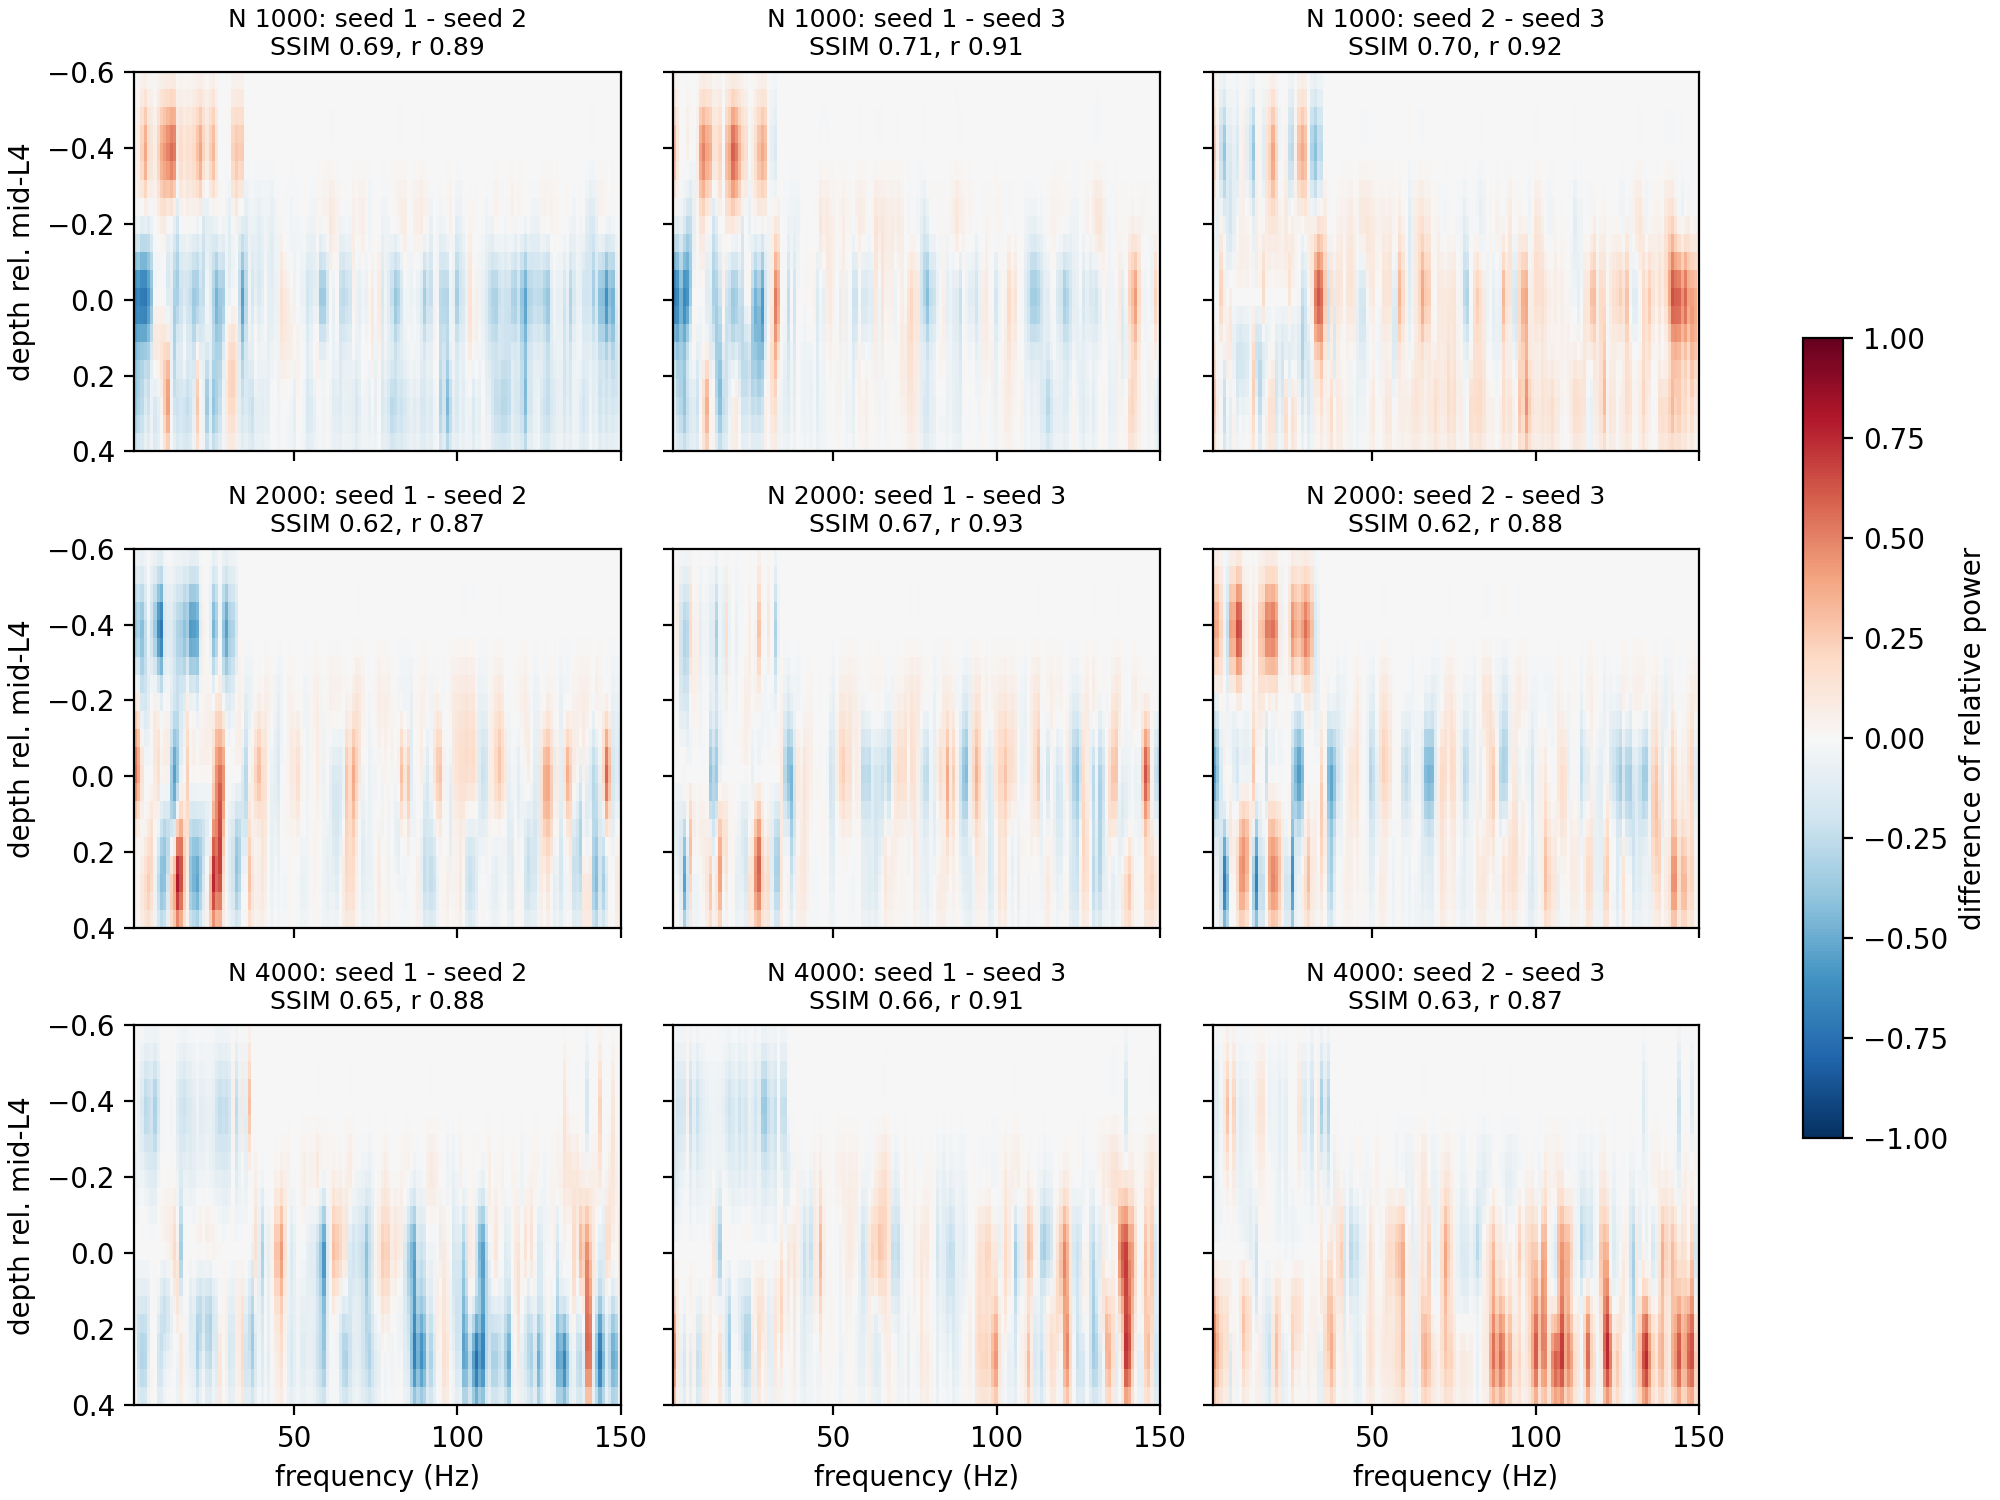
\includegraphics[width=\linewidth]{../../results/viz/paper_w6/seed_diff.png}}{\pendingbox{seed differences}}
\caption{Seed agreement on the finite-size ladder. Seed pairs: SSIM 0.62--0.71, pixel $r$ 0.87--0.93; each seed
against the observed map: SSIM 0.04--0.12, $r$ 0.20--0.43 (\texttt{results/viz/paper\_w6/seed\_diff.json}).}
\label{fig:seeds}
\end{figure}

\begin{figure}[tbp]
\centering
\panel{N1000 s1}{../../results/laminar_e2/lfs_n1000_s1_T8_motif.png}{0.32\linewidth}{missing}\hfill
\panel{N1000 s2}{../../results/laminar_e2/lfs_n1000_s2_T8_motif.png}{0.32\linewidth}{missing}\hfill
\panel{N1000 s3}{../../results/laminar_e2/lfs_n1000_s3_T8_motif.png}{0.32\linewidth}{missing}\\[0.8em]
\panel{N2000 s1}{../../results/laminar_e2/lfs_n2000_s1_T8_motif.png}{0.32\linewidth}{missing}\hfill
\panel{N2000 s2}{../../results/laminar_e2/lfs_n2000_s2_T8_motif.png}{0.32\linewidth}{missing}\hfill
\panel{N2000 s3}{../../results/laminar_e2/lfs_n2000_s3_T8_motif.png}{0.32\linewidth}{missing}\\[0.8em]
\panel{N4000 s1}{../../results/laminar_e2/sw_n4000_dens_k1_kd1_sst15_s1_T8_motif.png}{0.32\linewidth}{missing}\hfill
\panel{N4000 s2}{../../results/laminar_e2/lfs_n4000_s2_T8_motif.png}{0.32\linewidth}{missing}\hfill
\panel{N4000 s3}{../../results/laminar_e2/lfs_n4000_s3_T8_motif.png}{0.32\linewidth}{missing}
\caption{Finite-size ladder motif maps, one per $N$ and seed; scores in Table~\ref{tab:ladder}. Ladder rule (\texttt{results/laminar\_e2/lfs\_rule.json}): seed-mean
$r_\text{proto}$ 0.334, 0.387, 0.328 for $N$ = 1000, 2000, 4000; both smaller $N$ are within 2 SD of $N = 4000$ in
$r_\text{proto}$ but fail the 3 Hz peak test on the S unit (seed-mean S peak 8, 31, 43 Hz), so the T1 size is
$N = 4000$.}
\label{fig:s-ladder}
\end{figure}

\begin{table}[tbp]
\centering
\small
\begin{tabular}{lp{0.42\linewidth}ll}
\toprule
Test & Manipulation & Seal & Status \\
\midrule
T2 & every GABA weight $\times g$, $g \in \{0.25,\ldots,4\}$ & \path{SEAL_T2_T3.md} & sealed, not run \\
T3 & every unit's $N_\text{SOM}/N_\text{PV} \times s$, $s \in \{0.25,\ldots,4\}$ & \path{SEAL_T2_T3.md} & sealed, not run \\
T4 & PV or SOM silencing and $+50$ pA stimulation per unit & \path{SEAL_T4.md} & sealed, not run \\
T5 & VIP population & none & deferred (AdEx has no VIP) \\
\bottomrule
\end{tabular}
\caption{Sealed or planned tests not run for this report (seals in \texttt{docs/laminar\_motif/}).}
\label{tab:notrun}
\end{table}


\bibliographystyle{plainnat}
\bibliography{refs}

\end{document}
